%%%%%%%%%%%%%%%%%%%%%%%%%%%%%%%%%%%%%%%%%%%%%%%%%%%%%%%%%%%%%%%%%%%%%%
%% newminsetpresentation.tex
%% PhD Defence — From Scratch
%% Synthesised from: chapterconflict.tex, conflictmeat.tex,
%%   chaptercontract.tex, forwardtight.tex, forwardlooking2.tex,
%%   quantitativeviol.tex, qviol.tex
%%%%%%%%%%%%%%%%%%%%%%%%%%%%%%%%%%%%%%%%%%%%%%%%%%%%%%%%%%%%%%%%%%%%%%
\documentclass[9pt,aspectratio=169]{beamer}

\usepackage[T1]{fontenc}
\usepackage[utf8]{inputenc}
\usepackage[english]{babel}
\usepackage{amsmath,amssymb,mathtools}
\usepackage{stmaryrd}
\usepackage{xspace}
\usepackage{tikz}
\usetikzlibrary{arrows.meta,positioning,calc,fit,backgrounds,
  decorations.pathreplacing,patterns,patterns.meta,shapes.geometric,automata}
\usepackage{bm}
\usepackage{appendixnumberbeamer}

\usetheme{HLISP}

% ── Colour palette ────────────────────────────────────────────────
\definecolor{ConflictBlue}{RGB}{17,84,124}
\definecolor{ConflictGreen}{RGB}{43,122,83}
\definecolor{ConflictRed}{RGB}{178,53,52}
\definecolor{ConflictOrange}{RGB}{215,137,34}
\definecolor{ConflictGray}{RGB}{70,70,70}
\definecolor{SoftBlue}{RGB}{230,240,247}
\definecolor{SoftGreen}{RGB}{232,244,236}
\definecolor{SoftRed}{RGB}{248,233,232}
\definecolor{SoftOrange}{RGB}{250,240,226}

% ── Notation macros (self-contained, no \input{macros}) ───────────
\newcommand{\logic}[1]{\ensuremath{\mathsf{#1}}\xspace}
\newcommand{\TDDLfm}{\logic{\mu MTNL}}
\newcommand{\cDL}{\logic{TACNL}}
\newcommand{\Prog}{\ensuremath{\mathsf{Prog}}\xspace}
\newcommand{\repair}{\ensuremath{\blacktriangleright}}
\newcommand{\obl}[2][]{\mathbf{O}_{#1}(#2)}
\newcommand{\frb}[2][]{\mathbf{F}_{#1}(#2)}
\newcommand{\perm}[2][]{\mathbf{P}_{#1}(#2)}
\newcommand{\repit}[1]{\mathbf{Rep}(#1)}
\newcommand{\guard}[2][]{\lceil #1 \rceil #2}
\newcommand{\trig}[2][]{\langle\!\langle #1 \rangle\!\rangle #2}
\newcommand{\trace}[1]{\ensuremath{\langle #1 \rangle}\xspace}
\newcommand{\emptytrace}{\ensuremath{\trace{-}}}
\newcommand{\emptc}{\ensuremath{\epsilon_{C}}}
\newcommand{\nd}{\text{ and }}
\newcommand{\sor}{\text{ or }}
\newcommand{\is}{\ensuremath{\mathfrak{I}}}
\newcommand{\dpnf}{\ensuremath{\mathsf{DPNF}}}
\newcommand{\pnf}{\ensuremath{\mathsf{PNF}}}
\newcommand{\dnf}{\ensuremath{\mathsf{DNF}}}
\newcommand{\cd}{\ensuremath{\mathsf{C_\delta}}\xspace}
\newcommand{\Namb}{\ensuremath{\mathsf{CFR}}\xspace}
\newcommand{\pt}{\ensuremath{\mathsf{pt}}}
\newcommand{\mathcall}[1]{\text{\usefont{OMS}{cmsy}{m}{n}#1}}
\newcommand{\size}[1]{\vert #1\vert}
\newcommand{\LUCO}{\ensuremath{\mathrm{LUCO}}\xspace}
\newcommand{\LAP}{\ensuremath{\mathrm{LAP}}\xspace}
% Tight verdicts
\newcommand{\topt}{\top^t}
\newcommand{\bott}{\bot^t}
\newcommand{\topp}{\top^p}
\newcommand{\botp}{\bot^p}
\newcommand{\bottp}[1]{\mathbin{\bot^{t}_{#1}}}
\newcommand{\botpp}[1]{\mathbin{\bot^{p}_{#1}}}
% Semantic brackets
\newcommand{\satt}{\models_{\topt}}
\newcommand{\violt}{\models_{\bott}}
\newcommand{\presat}{\models_{?}}
\newcommand{\postsat}{\models_{\topp}}
\newcommand{\postviol}{\models_{\botp}}
\newcommand{\tightverdicts}{\ensuremath{\mathbb{V}_5}\xspace}
% Quantitative
\newcommand{\qsem}[1]{\llbracket #1 \rrbracket_{\text{qviol}}}
\newcommand{\qblame}[1]{\llbracket #1 \rrbracket_{\text{qblame}}}
\newcommand{\qscore}{\ensuremath{\mathsf{Score}}}
\newcommand{\qmc}{\ensuremath{\mathsf{QMC}}}
\newcommand{\qbm}{\ensuremath{\mathsf{QBM}}}
\newcommand{\LH}{\ensuremath{\mathsf{LH}}}
\newcommand{\bmc}{\ensuremath{\mathsf{BMC}}}
\newcommand{\tsmc}{\ensuremath{\mathsf{TSMC}}}
\newcommand{\rrcs}[1]{\ensuremath{\mathsf{RRC}\!\left(#1\right)}\xspace}
\newcommand{\CPM}{\ensuremath{\mathsf{CPM}}\xspace}
% Actions
\newcommand{\PAY}{\ensuremath{\mathsf{PAY\_R}}\xspace}
\newcommand{\PAYF}{\ensuremath{\mathsf{PAY\_F}}\xspace}
\newcommand{\OCC}{\ensuremath{\mathsf{OCC}}\xspace}
\newcommand{\notifterm}{\ensuremath{\mathsf{Notif\_T}}}
\newcommand{\delAtGate}{\ensuremath{\mathsf{dag}}\xspace}
\newcommand{\delAtPark}{\ensuremath{\mathsf{dap}}\xspace}
\newcommand{\pickU}{\ensuremath{\mathsf{pick}}\xspace}
\newcommand{\DC}{\ensuremath{\mathsf{DC}}\xspace}
\newcommand{\SR}{\ensuremath{\mathsf{SR}}\xspace}
\newcommand{\MA}{\ensuremath{\mathsf{MA}}\xspace}
\newcommand{\UC}{\ensuremath{\mathsf{UC}}\xspace}
\newcommand{\ob}[2]{\ensuremath{O^{#1}\,#2}}
\newcommand{\forbb}[2]{\ensuremath{F^{#1}\,#2}}
\newcommand{\mydef}{\mathrel{\overset{\makebox[0pt]{\mbox{\normalfont\tiny\sffamily def}}}{=}}}

\setbeamertemplate{itemize item}{\color{uzlmain}$\blacktriangleright$}
\setbeamertemplate{itemize subitem}{\color{uzlmain}$\bullet$}

\title[Dissertation Defense]{Formal Modeling and Analysis of Metric-Timed and\\Multi-Agent Normative Specifications of Actions}

\institute[University of Lübeck]{Oral examination for the dissertation submitted to obtain\\ the Dr. rer. nat degree}


\begin{document}

% =====================================
% SLIDE 1 — Title
% =====================================
\begin{frame}
  \titlepage
  \vspace{-2mm}
  \begin{center}
    \small
    \renewcommand{\arraystretch}{1.3}
    
  \end{center}
\end{frame}




\begin{frame}{Motivation: The Cost of Manual Compliance}
  \begin{columns}[T,totalwidth=\textwidth]
  \begin{column}{0.48\textwidth}
  \onslide<1->{
    \begin{block}{What are Normative Specifications?}
      \small 
      \begin{itemize}
        \item A normative specification is a document or clause that outlines mandatory requirements, technical standards, or protocols that must be followed for compliance. 
        \item Contracts, laws, and regulations are examples of normative specifications.
      \end{itemize}
    \end{block}
  }
 
  \vspace{2mm}

  \end{column}
  \begin{column}{0.52\textwidth}
  \centering
    \onslide<2->{
    \begin{block}{The Scaling Problem}
      \small 
      \begin{itemize}
        \item Regulatory burden costs the global economy \alert{trillions of dollars} annually:\textbf{3.5 \% of Europe's GDP}.\\
        \item The manual management of normative specifications is a time-consuming and error-prone process.
      \end{itemize}
    \end{block}
  }
  \end{column}
  \end{columns}
   \onslide<3->{
    \begin{block}{The Solution: Legaltech }
    \begin{itemize}
      \item Legaltech, or legal technology, refers to the application of software and digital tools to provide legal services and support the justice system.
    \end{itemize}
    \end{block}
  }
\end{frame}

% ---------------- Slide 3 ----------------
\begin{frame}{Legaltech between probabilistic AI and formal methods}
\begin{columns}[T,totalwidth=\textwidth]
\begin{column}{0.48\textwidth}
\onslide<2->{
  \begin{block}{LLM in legaltech}
    \small 
    According to a new survey of over 200 inhouse and law firm lawyers \footnote{https://www.artificiallawyer.com/2026/04/07/}, \alert{69.7\%} of legal outputs still require targeted edits or extensive rework.
  \end{block}
}
\vspace{2mm}
\onslide<2->{
  \begin{block}{The Formal Methods Alternative}
    \small 
    Legislation as code aims to treat specifications as mathematical objects, where questions about behavior yield provable verdicts rather than statistical guesses.
  \end{block}
}
\end{column}
\begin{column}{0.52\textwidth}
\centering
\vspace{6mm}
\onslide<1->{
  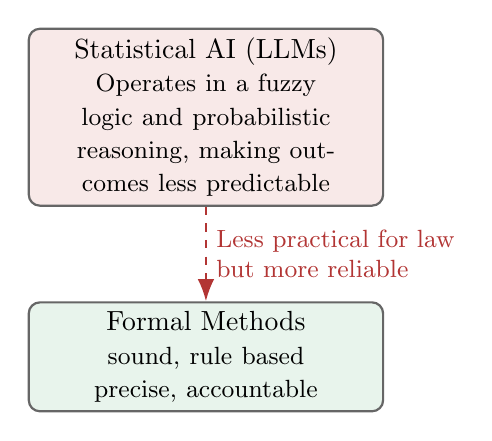
\begin{tikzpicture}[
    box/.style={rounded corners=4pt, draw=black!60, thick, minimum width=4.5cm, minimum height=1.1cm, align=center},
    arr/.style={-{Latex[length=2.8mm]}, thick, black!65}
  ]
  \node[box, fill=SoftRed, text width=4.2cm] (ai) {Statistical AI (LLMs)\\ \small Operates in a fuzzy logic and probabilistic reasoning, making outcomes less predictable};
  \node[box, fill=SoftGreen, text width=4.2cm, below=12mm of ai] (fm) {Formal Methods\\ \small sound, rule based precise, accountable};
  \draw[arr, dashed, ConflictRed] (ai) -- node[right, align=left, font=\small] {Less practical for law \\ but more reliable} (fm);
  \end{tikzpicture}
}
\end{column}
\end{columns}
\end{frame}

% =====================================
% SLIDE 2 — Thesis Vision & Research Gap
% =====================================
\begin{frame}{Thesis Vision: The two families of formal methods applied to Normative reasoning}

\centering
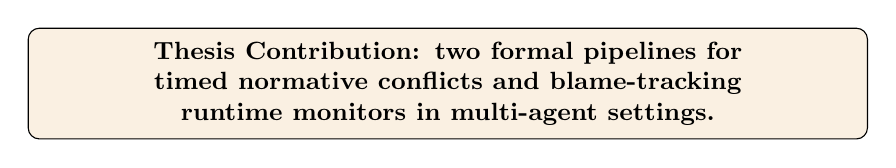
\begin{tikzpicture}
  \node[draw,rounded corners,fill=SoftOrange,text width=0.85\textwidth,align=center,inner sep=5pt,font=\small\bfseries] {
  Thesis Contribution: two formal pipelines for timed normative conflicts and blame-tracking runtime monitors in multi-agent settings.
  };
\end{tikzpicture}
\vspace{4mm}
\begin{columns}[T]
  \begin{column}{0.48\textwidth}
    \begin{block}{Before Adoption \textemdash\ Static Analysis}
      \small
      Reasoning about conflicts in metric timed normative specifications.
    \medskip

      \textbf{Problem:}  Conflicting norms \emph{hide} inside complex temporal conditions, we suggest a novel characterization of timed normative conflicts.
    \end{block}
  \end{column}
  \begin{column}{0.48\textwidth}
    \begin{block}{During Enforcement \textemdash\ Runtime Monitoring}
      \small
     Perpetual Blame Monitoring  in multi-agent contracts.
      
      \medskip

      \textbf{Problem:}  Contracts specify collaborative multi-agent behavior that may run indefinitely, requiring:
      \begin{itemize}\setlength\itemsep{1pt}
        \item Monitoring that also tracks \emph{obstructions}, not only non-performance, and
        \item Per-agent \emph{cumulative blame attribution}  over the whole contract execution.
      \end{itemize}
    \end{block}
  \end{column}
\end{columns}
\end{frame}

% =====================================
% PART I SEPARATOR
% =====================================
{
\setbeamercolor{background canvas}{bg=ConflictBlue}
\begin{frame}[plain]
  \vfill
  \centering
  \textcolor{white}{\Huge\bfseries Part I}\\[6mm]
  \textcolor{white!85}{\Large Reasoning about Metric-Timed Normative Conflicts }\\[3mm]
  \textcolor{white!70}{\large Micro Metric-Timed Normative Logic $\TDDLfm$}
  \vfill
\end{frame}
}



\begin{frame}{Intuitive understanding of normative conflicts}
\onslide<1->{
  \begin{block}{The Fundamental Intuition}
    \small
    \emph{``Normative conflicts occur when complying with one norm can lead to noncompliance with another.''}
    \vspace{1mm}
    
    \raggedleft\footnotesize \color{gray} --- H. Kelsen, \textit{General Theory of Norms} (1991)
  \end{block}
}
\vspace{3mm}
\onslide<2->{
  \begin{block}{Deontic Conflicts in Dynamic Settings over time}
    \small
    \emph{``A deontic conflict occurs when a set of obligations is jointly unsatisfiable over time, meaning that no trace can be constructed that complies with every obligation in the set.''}
    \vspace{1mm}
    
    \raggedleft\footnotesize \color{gray} --- S. Colombo Tosatto et al., \textit{DEON} (2014)
  \end{block}
}
\vspace{3mm}
\onslide<3->{
  \begin{block}{Conflicts via Satisfiability}
    \small
    \emph{``A normative conflict occurs when triggering a normative rule, either always or in some feasible situation, inevitably leads to the violation of one or more rules, because the rule set imposes incompatible requirements.''}
    \vspace{1mm}
    
    \raggedleft\footnotesize \color{gray} --- N. Feng et al., \textit{ICSE} (2024)
  \end{block}
}
\end{frame}


% % =====================================
% % SLIDE 3 — Research Questions (Conflict)
% % =====================================
% \begin{frame}{Research Questions \textemdash\ Conflict Analysis}
% \begin{enumerate}[\bfseries RQ1.]
%   \item \textbf{Unsatisfiability and Conflict:}\quad Is every unsatisfiable formula necessarily a conflict?  Conversely, does a conflict imply unsatisfiability?

%   \medskip
%   \item \textbf{Conflict Quantification:}\quad Can we define a \emph{measure for the degree of conflict} within a specification?

%   \medskip
%   \item \textbf{Semantics-Preserving Resolution:}\quad Can we always resolve conflicts without altering the intended compliant behaviours. What are the properties of such resolutions?
% \end{enumerate}


% \end{frame}


% =====================================
% SLIDE 3 — Conflict Motivation
% ===================================
\begin{frame}{Motivation: Inpterpreting Timed norms as a Planning Problem}
\begin{columns}[T]
  \begin{column}{0.52\textwidth}
    \small
    \textbf{Use case:} Goods delivery to a harbour.

    \begin{itemize}
      \item \DC: Deliver between 09:00--16:00 to gate \textbf{or} parking.
      \item \SR: Parking \textbf{prohibited} 10:00--14:00.
      \item \MA: Gate \textbf{prohibited} 02:00--04:00, 08:00--24:00.
    \end{itemize}


    Conflicts are not logical contradictions in isolation: they arise from \emph{overlapping activation windows} and \emph{single-action capacity}.

    \medskip
    \textbf{Conflict at a specific time point t:}
    \begin{enumerate}
      \item \textcolor{ConflictRed}{\textbf{Deontic:}} Two contradictory obligations/prohibitions specified at the same t.
      \item \textcolor{ConflictOrange}{\textbf{Ontic:}} Two obliged actions cannot be performed at the same time t.
    \end{enumerate}

   
  \end{column}
  \begin{column}{0.45\textwidth}
    \centering
    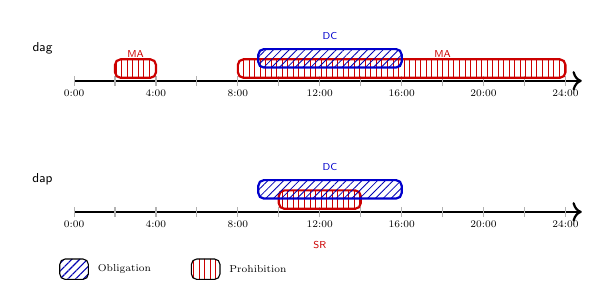
\begin{tikzpicture}[scale=0.52,transform shape]
      \begin{scope}[x=0.5cm, shift={(1cm,0)}]
        % Layout parameters
        \def\laneH{0.45}
        \def\offset{0.25}
        \def\yshiftText{0.6}
        \def\rectShift{0.3}
        \def\ygate{1.6}
        \def\ypark{-1.6}

        % Styles
        \tikzset{
          obl/.style={draw=blue!80!black, line width=0.8pt, rounded corners=2pt,
            pattern={Lines[angle=45,distance=2pt,line width=0.3pt]},
            pattern color=blue!70!black, fill opacity=1},
          proh/.style={draw=red!80!black, line width=0.8pt, rounded corners=2pt,
            pattern={Lines[angle=90,distance=2pt,line width=0.3pt]},
            pattern color=red!80!black, fill opacity=1},
          tick/.style={gray!60, line width=0.4pt}
        }

        % Gate timeline
        \draw[thick,->] (0,\ygate) -- (24.8,\ygate);
        \foreach \t in {0,2,...,24} {
          \draw[tick] (\t,\ygate-0.12) -- (\t,\ygate+0.12);
        }
        \foreach \t in {0,4,8,12,16,20,24} {
          \node[below=3pt, font=\scriptsize] at (\t,\ygate) {\t:00};
        }

        % Park timeline
        \draw[thick,->] (0,\ypark) -- (24.8,\ypark);
        \foreach \t in {0,2,...,24} {
          \draw[tick] (\t,\ypark-0.12) -- (\t,\ypark+0.12);
        }
        \foreach \t in {0,4,8,12,16,20,24} {
          \node[below=3pt, font=\scriptsize] at (\t,\ypark) {\t:00};
        }

        % Timeline labels
        \node[anchor=east, font=\small] at (-0.8,\ygate+0.8) {\delAtGate};
        \node[anchor=east, font=\small] at (-0.8,\ypark+0.8) {\delAtPark};

        % Gate intervals
        \def\GateProhSmallA{2} \def\GateProhSmallB{4}
        \def\GateProhA{8}      \def\GateProhB{24}
        \def\GateOblA{9}       \def\GateOblB{16}

        % Gate prohibitions
        \path[proh] (\GateProhSmallA,\ygate+\rectShift-\laneH/2)
          rectangle (\GateProhSmallB,\ygate+\rectShift+\laneH/2);
        \path[proh] (\GateProhA,\ygate+\rectShift-\laneH/2)
          rectangle (\GateProhB,\ygate+\rectShift+\laneH/2);
        % Gate obligation
        \path[obl]  (\GateOblA,\ygate+\rectShift+\offset-\laneH/2)
          rectangle (\GateOblB,\ygate+\rectShift+\offset+\laneH/2);

        % Gate labels
        \node[blue!80!black, font=\scriptsize,yshift=+0.2cm]
          at ({(\GateOblA+\GateOblB)/2},\ygate+\rectShift+\offset+\laneH/1.3) {\DC};
        \node[red!80!black, font=\scriptsize,yshift=1.3cm,xshift=1cm]
          at ({(\GateProhA+\GateProhB)/2},\ygate+\rectShift-\laneH/1.3-\yshiftText) {\MA};
        \node[red!80!black, font=\scriptsize,yshift=+1.3cm]
          at ({(\GateProhSmallA+\GateProhSmallB)/2},\ygate+\rectShift-\laneH/1.3-\yshiftText) {\MA};

        % Park intervals
        \def\ParkOblA{9}   \def\ParkOblB{16}
        \def\ParkProhA{10} \def\ParkProhB{14}

        % Park prohibition
        \path[proh] (\ParkProhA,\ypark+\rectShift-\laneH/2)
          rectangle (\ParkProhB,\ypark+\rectShift+\laneH/2);
        % Park obligation
        \path[obl]  (\ParkOblA,\ypark+\rectShift+\offset-\laneH/2)
          rectangle (\ParkOblB,\ypark+\rectShift+\offset+\laneH/2);

        % Park labels
        \node[blue!80!black, font=\scriptsize,yshift=+0.2cm]
          at ({(\ParkOblA+\ParkOblB)/2},\ypark+\rectShift+\offset+\laneH/1.3) {\DC};
        \node[red!80!black, font=\scriptsize,yshift=-0.2cm]
          at ({(\ParkProhA+\ParkProhB)/2},\ypark+\rectShift-\laneH/1.5-\yshiftText) {\SR};

        % Legend
        \begin{scope}[shift={(0,-3.0)}]
          \node[draw, rounded corners=2pt,
                pattern={Lines[angle=45,distance=2pt,line width=0.4pt]},
                pattern color=blue!70!black,
                minimum height=5mm, minimum width=7mm] (legO) {};
          \node[right=1mm of legO, font=\scriptsize] {Obligation};

          \node[draw, rounded corners=2pt,
                pattern={Lines[angle=90,distance=2pt,line width=0.4pt]},
                pattern color=red!80!black,
                minimum height=5mm, minimum width=7mm, right=25mm of legO] (legF) {};
          \node[right=1mm of legF, font=\scriptsize] {Prohibition};
        \end{scope}
      \end{scope}
    \end{tikzpicture}
   \medskip \medskip
    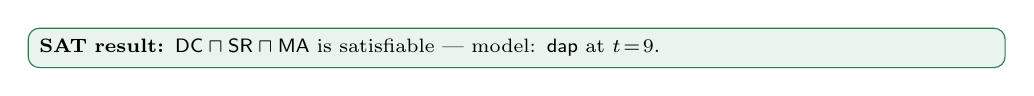
\begin{tikzpicture}
      \node[draw=ConflictGreen,rounded corners,fill=SoftGreen,text width=\columnwidth,align=left,inner sep=4pt,font=\scriptsize] {
      \textbf{SAT result:} $\DC \sqcap \SR \sqcap \MA$ is satisfiable~--- model: $\delAtPark$ at $t\!=\!9$.
      };
    \end{tikzpicture}
  \end{column}
\end{columns}

\end{frame}


% \begin{frame}{Syntactic definition and analysis of conflicts in $\TDDLfm$ }
% \begin{center}
% \begin{tikzpicture}[
%   node distance=10mm and 14mm,
%   box/.style={rectangle, draw, rounded corners, text width=26mm, align=center, minimum height=10mm, font=\scriptsize},
%   arr/.style={-{Stealth[round]}, thick}
% ]
%   \node[box, fill=SoftBlue] (spec) {Normative Spec.\\$\phi \in \TDDLfm$};
%   \node[box, fill=SoftBlue, right=of spec] (pnf) {Punctual NF\\$\pnf(\phi,k)$};
%   \node[box, fill=SoftBlue, right=of pnf] (dpnf) {Disjunctive PNF\\$\dpnf(\phi,k)$};
%   \node[box, fill=SoftRed, below=8mm of dpnf] (detect) {Conflict\\Detection};
%   \node[box, fill=SoftOrange, left=of detect] (density) {Conflict Density\\$\cd(\phi) \in [0,1]$};
%   \node[box, fill=SoftGreen, left=of density] (cfr) {Conflict-Free\\Rewriting $\Namb(\phi)$};

%   \draw[arr] (spec) -- (pnf);
%   \draw[arr] (pnf) -- (dpnf);
%   \draw[arr] (dpnf) -- (detect);
%   \draw[arr] (detect) -- (density);
%   \draw[arr] (density) -- (cfr);
% \end{tikzpicture}
% \end{center}

% \smallskip
% \begin{columns}[T]
% \begin{column}{0.48\textwidth}
%   \small
%   \begin{itemize}
%     \item Action-based trace semantics: each timed event carries \emph{exactly one action}.
%     \item Time constraints encoded as \textbf{canonical interval sets} $\is$.
%     \item Normalization decomposes intervals into \emph{punctual atoms}.
%   \end{itemize}
% \end{column}
% \begin{column}{0.48\textwidth}
%   \small
%   \begin{itemize}
%     \item Conflict detection via pattern matching on product terms of the \dpnf.
%     \item Structural invariants literal ancestor preservation to ensure no spurious conflicts are introduced.
%     \item Exponential worst-case blowup $\Rightarrow$ mitigated by  conflict calculus.
%   \end{itemize}
% \end{column}
% \end{columns}
% \end{frame}


% \begin{frame}{semantic characterization of conflicts in $\TDDLfm$ }
% \begin{center}

% \end{frame}
% =====================================
% SLIDE 5 — Methodology (Conflict)
% =====================================
\begin{frame}{Syntactic definition and analysis of conflicts in $\TDDLfm$ }
\small
\begin{columns}[T]
\begin{column}{0.48\textwidth}
  \textbf{Punctual Conflicts}
  \medskip

  Conflicts are identified syntactically at individual time points $t$:
  \begin{enumerate}
    \item \textbf{P-Deon-Conf:}
    $ \ob{\{[t,t]\}}{a} \sqcap \forbb{\{[t,t]\}}{a} $
    \item \textbf{P-Ont-Conf:}
    $ \ob{\{[t,t]\}}{a} \sqcap \ob{\{[t,t]\}}{b} $
  \end{enumerate}
  \vspace{2mm}
  % \emph{Any Formula \textit{syntactically formed} by these patterns is conflicting.}
  \vspace{1mm}
 As literals in formulas are not always punctual, we introduce the \dpnf~  that decomposes time intervals into punctual atoms, allowing us to detect conflicts at the punctual level.
\end{column}

\begin{column}{0.48\textwidth}
  \textbf{The Syntactic Analysis Pipeline}
  
  \vspace{2mm}
  \begin{center}
  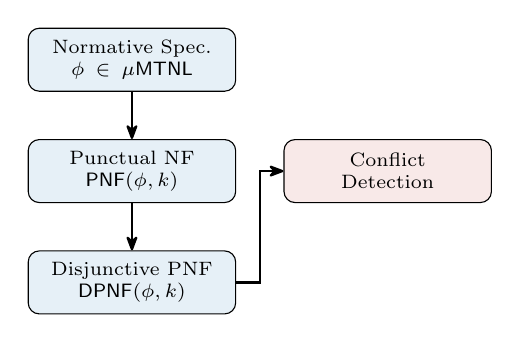
\begin{tikzpicture}[
    node distance=6mm and 6mm,
    box/.style={rectangle, draw, rounded corners, text width=24mm, align=center, minimum height=8mm, font=\scriptsize},
    arr/.style={-{Stealth[round]}, thick}
  ]
    \node[box, fill=SoftBlue] (spec) {Normative Spec.\\$\phi \in \TDDLfm$};
    \node[box, fill=SoftBlue, below=of spec] (pnf) {Punctual NF\\$\pnf(\phi,k)$};
    \node[box, fill=SoftBlue, below=of pnf] (dpnf) {Disjunctive PNF\\$\dpnf(\phi,k)$};
    \node[box, fill=SoftRed, right=of pnf] (detect) {Conflict\\Detection};
    
    \draw[arr] (spec) -- (pnf);
    \draw[arr] (pnf) -- (dpnf);
    \draw[arr] (dpnf.east) -- ++(0.3,0) |- (detect.west);
  \end{tikzpicture}
  \end{center}
  \vspace{1mm}
  \begin{itemize}
    \item Structural invariants literal ancestor preservation.
    \item Exponential worst-case blow-up in the size of $\dpnf(\phi,x)$.
  \end{itemize}
\end{column}
\end{columns}
\end{frame}

\begin{frame}{Example of conflict analysis}
\begin{table}
    \centering
    \renewcommand{\arraystretch}{1}
    \resizebox{\textwidth}{!}{%
    \begin{tabular}{|l|p{12cm}|c|}
    \hline
    \textbf{Step} & \textbf{Value} & \textbf{Size} \\
    \hline
    $\phi$ 
    & 
    $\ob{\{[1,2]\}}{\delAtGate} \sqcap \forbb{\{[2,5]\}}{\delAtGate} \sqcap \ob{\{[1,2]\}}{\pickU}$
    & 14 \\
    \hline
    $\pnf(\phi,2)$ 
    & 
    $\left( \ob{\{[1,1]\}}{\delAtGate} \sqcup \ob{\{[2,2]\}}{\delAtGate} \right) 
    \sqcap 
    \left( \forbb{\{[2,2]\}}{\delAtGate} \sqcap \forbb{\{[3,5]\}}{\delAtGate} \right)
    \sqcap 
    \left( \ob{\{[1,1]\}}{\pickU} \sqcup \ob{\{[2,2]\}}{\pickU} \right)$
    & 33 \\
    \hline
    $D\pnf(\phi,2))$ 
    & 
    $
    \begin{aligned}
    \left(
        \ob{\{[1,1]\}}{\delAtGate}
        \sqcap \forbb{\{[2,2]\}}{\delAtGate}
        \sqcap \forbb{\{[3,5]\}}{\delAtGate}
        \sqcap \ob{\{[1,1]\}}{\pickU}
      \right)\,\underline{pt_1}
      \\
      \sqcup\;
      \left(
        \ob{\{[1,1]\}}{\delAtGate}
        \sqcap \forbb{\{[2,2]\}}{\delAtGate}
        \sqcap \forbb{\{[3,5]\}}{\delAtGate}
        \sqcap \ob{\{[2,2]\}}{\pickU}
      \right)\,\underline{pt_2}
      \\
      \sqcup\;
      \left(
        \ob{\{[2,2]\}}{\delAtGate}
        \sqcap \forbb{\{[2,2]\}}{\delAtGate}
        \sqcap \forbb{\{[3,5]\}}{\delAtGate}
        \sqcap \ob{\{[1,1]\}}{\pickU}
      \right)\,\underline{pt_3}
      \\
      \sqcup\;
      \left(
        \ob{\{[2,2]\}}{\delAtGate}
        \sqcap \forbb{\{[2,2]\}}{\delAtGate}
        \sqcap \forbb{\{[3,5]\}}{\delAtGate}
        \sqcap \ob{\{[2,2]\}}{\pickU}
      \right)\,\underline{pt_4}
    \end{aligned}
    $
    & 76 \\
    \hline
    $\mathcall{PC}(\phi)$ 
    & 
    $
    \begin{aligned}
    &\big(\pt_1,\{\ob{\{[1,1]\}}{\delAtGate} \sqcap \ob{\{[1,1]\}}{\pickU}\}\big), \\
    &\big(\pt_3,\{\ob{\{[2,2]\}}{\delAtGate} \sqcap \forbb{\{[2,2]\}}{\delAtGate} \}\big)\\
    &\big(\pt_4,\{\ob{\{[2,2]\}}{\delAtGate} \sqcap \forbb{\{[2,2]\}}{\delAtGate}, \ob{\{[2,2]\}}{\delAtGate} \sqcap  \ob{\{[2,2]\}}{\pickU}\} \big)
    \end{aligned}
    $
    & -- \\
    \hline
    \end{tabular}%
    }
    %\caption{Normal form analysis with sizes for $\phi := \ob{\{[1,2]\}}{\delAtGate} \sqcap \forbb{\{[2,5]\}}{\delAtGate} \sqcap \ob{\{[1,2]\}}{\pickU}$.}
    \label{table:conflict-analysis}
    \end{table}
\end{frame}

% % =====================================
% % SLIDE 5b — Semantic Characterization
% % =====================================
% \begin{frame}{semantic characterization of conflicts in $\TDDLfm$ }
% \small
% \textbf{From Syntax to Semantics:} Are these syntactic patterns exact?

% \vspace{3mm}
% \begin{columns}[T]
% \begin{column}{0.50\textwidth}
%   \begin{block}{Punctual MUS (Minimal Unsatisfiable Subset)}
%     At the level of the $\dpnf$, each product term acts as a local scenario. A \textbf{Punctual MUS} is the smallest set of punctual literals inside a product term that:
%     \begin{enumerate}[(i)]
%       \item cannot be jointly satisfied by any valid trace.
%       \item becomes satisfiable if any single literal is removed.
%     \end{enumerate}
%   \end{block}
% \end{column}
% \begin{column}{0.46\textwidth}
%   \textbf{Key Results:}
%   \begin{itemize}\setlength\itemsep{2pt}
%     \item Isolated punctual obligations/prohibitions are \emph{always} satisfiable.
%     \item The only two minimal combinations that fail are exactly the syntactic \textbf{P-Deon-Conf} and \textbf{P-Ont-Conf} patterns.
%     \item \textbf{Global Unsatisfiability:} A formula $\phi$ is globally unsatisfiable iff \emph{every} product term in $\dpnf(\phi)$ contains a Punctual MUS.
%   \end{itemize}
% \end{column}
% \end{columns}

% \vspace{4mm}
% \centering
% \begin{tikzpicture}
%   \node[draw=ConflictGreen,rounded corners,fill=SoftGreen,text width=0.9\textwidth,align=center,inner sep=4pt,font=\small] {
%   \textbf{Conclusion:} Syntactic punctual conflicts coincide perfectly with semantic Punctual MUSes. This provides exact unsatisfiability assessment and explainability.
%   };
% \end{tikzpicture}
% \end{frame}

% =====================================
% SLIDE 6 — Answering RQ1–RQ3
% =====================================
\begin{frame}{Key results through conflict density}
\small
\begin{columns}[T]
  \begin{column}{0.32\textwidth}
  \begin{block}{Conflict Density}
    \[
    \cd(\phi) := \frac{|\text{CPT in } \dpnf(\phi)|}{|\text{PT in } \dpnf(\phi)|}
    \]
    \begin{itemize}\setlength\itemsep{2pt}
      \item $\cd = 0$: conflict-free.
      \item $\cd = 1$: fully conflicting.
      \item Use case: $\cd(\UC) = 75\%$.
    \end{itemize}
  \end{block}
\end{column}
\begin{column}{0.32\textwidth}
  \begin{block}{Conflicts vs unsatisfiability}
    \centering
    
    
    

    \raggedright
    \textbf{Key results:}
    \begin{itemize}\setlength\itemsep{2pt}
      \item $\phi$ is unsat $\;\Longleftrightarrow\;$ $\cd(\phi) = 1$
      \item Punctual conflicts $\equiv$ Minimal unsatisfiable set (MUS) in the \dpnf.
    \end{itemize}
  \end{block}
\end{column}

\begin{column}{0.32\textwidth}
  \begin{block}{Conflict-Free Rewriting}
    If $\cd(\phi) < 1$:
    
      $\quad \exists\;\phi' \equiv \phi,\quad \cd(\phi') = 0$
    
    \begin{itemize}\setlength\itemsep{2pt}
      \item Prune conflicting terms.
      \item May return a very big size repaired formula.
      \item Conflict calculus for choosing to partially repair the formula.
    \end{itemize}
  \end{block}
\end{column}
\end{columns}
\end{frame}

% =====================================
% SLIDE 7 — The Overall Framework (Conflict)
% =====================================
\begin{frame}{Sound and complete Conflict Analysis \& Resolution Framework}
\begin{center}
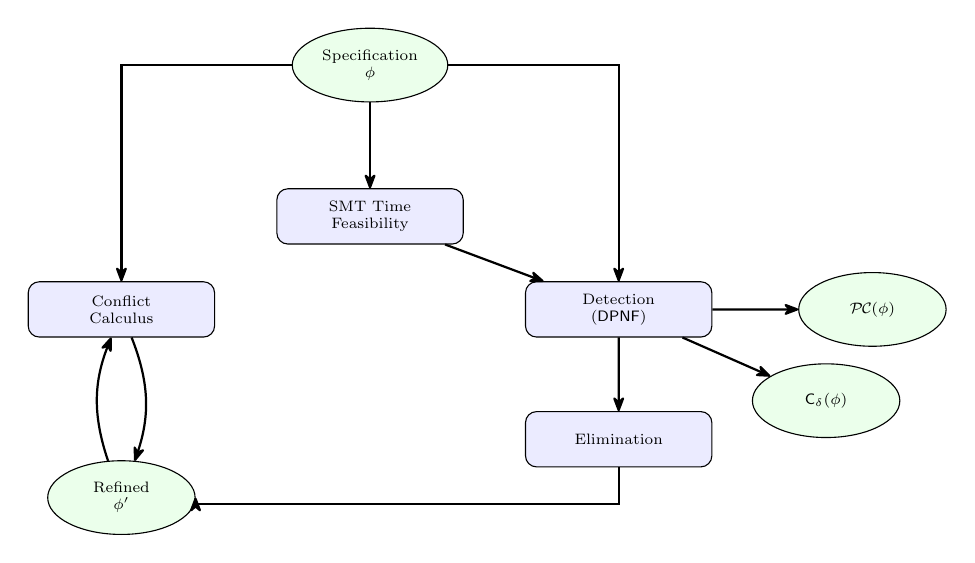
\begin{tikzpicture}[
  node distance=14mm and 16mm,
  rect/.style={rectangle, draw, rounded corners, text width=28mm, align=center, minimum height=9mm, fill=blue!8, font=\scriptsize},
  ell/.style={ellipse, draw, minimum width=24mm, minimum height=12mm, align=center, fill=green!8, font=\scriptsize},
  arr/.style={-{Stealth[round]}, thick},
  scale=0.78, transform shape
]
  \node[ell] (spec) {Specification\\$\phi$};
  \node[rect, below=of spec] (smt) {SMT Time\\Feasibility};
  \node[rect, below left=6mm and 10mm of smt] (calc) {Conflict\\Calculus};
  \node[rect, below right=6mm and 10mm of smt] (det) {Detection\\(\dpnf)};
  \node[rect, below=12mm of det] (elim) {Elimination};
  \node[ell, right=14mm of det] (pc) {$\mathcall{PC}(\phi)$};
  \node[ell, below right=6mm and 10mm of det] (cdens) {$\cd(\phi)$};
  \node[ell, below=20mm of calc] (ref) {Refined\\$\phi'$};

  \draw[arr] (spec) -- (smt);
  \draw[arr] (spec.west) -| (calc.north);
  \draw[arr] (spec.east) -| (det.north);
  \draw[arr] (smt) -- (det);
  \draw[arr] (det) -- (pc);
  \draw[arr] (det) -- (elim);
  \draw[arr] (det) -- (cdens);
  \draw[arr] (elim.south) -- ++(0,-0.6) -| (ref.east);
  \draw[arr] (calc) to[bend left=20] (ref);
  \draw[arr] (ref) to[bend left=20] (calc);
\end{tikzpicture}
\end{center}
\end{frame}

% =====================================
% PART II SEPARATOR
% =====================================
{
\setbeamercolor{background canvas}{bg=ConflictGreen}
\begin{frame}[plain]
  \vfill
  \centering
  \textcolor{white}{\Huge\bfseries Part II}\\[6mm]
  \textcolor{white!85}{\Large  Reasoning about Blame in Multi-Party Collaborative Contracts }\\[3mm]
  \textcolor{white!70}{\large Two-Agent Collaborative Normative Logic \cDL}
  \vfill
\end{frame}
}

%todo 7 slides for part II: 

% =====================================
% PART II — Slide 1
% =====================================
\begin{frame}{Challenges in Monitoring Multi-Party open-ended Contracts}
\small
\begin{columns}[T,totalwidth=\textwidth]
  \begin{column}{0.49\textwidth}
    \begin{block}{Challenges}
      \begin{itemize}
        \item Contract assign a duty to each party, but the outcome depends on their joint behavior.
        \item A violation may activate a reparation duty rather than a simple failure.
        \item Contracts are open-ended: they may be terminated or repeated indefinitely.
      \end{itemize}
    \end{block}
  \end{column}
\begin{column}{0.49\textwidth}
  \begin{block}{Running use case: rental contract}
    \begin{itemize}
      \item Tenant must pay rent every month.
      \item Missed rent payement activates a late-fee reparation.
      \item Landlord must guarantee occupancy.
      \item Payement and occupency are repeated in a montly basis until a termination notification is submitted.
    \end{itemize}
  \end{block}
\end{column}

\end{columns}

\vspace{2mm}
\begin{center}
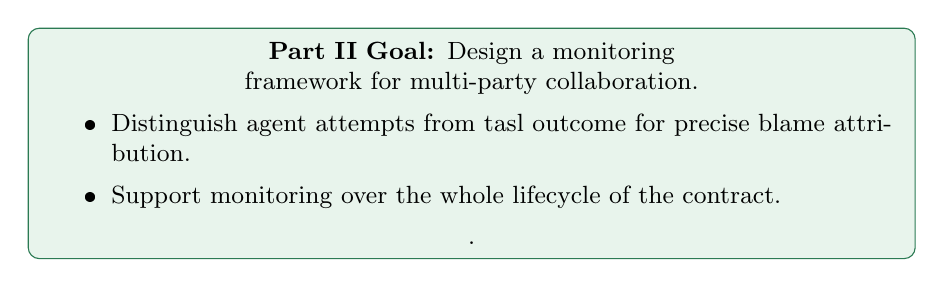
\begin{tikzpicture}
  \node[draw=ConflictGreen,rounded corners,fill=SoftGreen,text width=0.9\textwidth,align=center,inner sep=5pt,font=\small] {
  \textbf{Part II Goal:} Design a monitoring framework for multi-party collaboration.\begin{itemize}
    \item Distinguish agent  attempts from tasl outcome for precise blame attribution.
    \item Support monitoring over the whole lifecycle of the contract.
  \end{itemize}.
  };
\end{tikzpicture}
\end{center}
\end{frame}

% =====================================
% PART II — Slide 2
% =====================================
% \begin{frame}{Attempt-Based Interaction Model}
% \small
% \begin{center}
% \begin{tikzpicture}[
%   box/.style={rounded corners=4pt, draw=black!60, thick, minimum width=3.15cm, minimum height=1.2cm, align=center, text width=3cm},
%   arr/.style={-{Latex[length=2.8mm]}, thick, black!65}
% ]
%   \node[box, fill=SoftBlue] (timed) {Metric-timed traces\\$\tau_1,\tau_2$\\\footnotesize who acted and when};
%   \node[box, fill=SoftOrange, right=8mm of timed] (periodic) {Periodic set traces\\$\pi_1,\pi_2$\\\footnotesize monthly aggregation};
%   \node[box, fill=SoftGreen, right=8mm of periodic] (tagged) {Tagged collaboration traces\\$\pi_1^C,\pi_2^C$\\\footnotesize attempts are preserved};
%   \node[box, fill=SoftRed, right=8mm of tagged] (succ) {Derived success\\$\mathrm{Succ}(\pi_1^C,\pi_2^C)$\\\footnotesize joint outcome only};
%   \draw[arr] (timed) -- (periodic);
%   \draw[arr] (periodic) -- (tagged);
%   \draw[arr] (tagged) -- (succ);
% \end{tikzpicture}
% \end{center}

% \vspace{2mm}
% \begin{columns}[T,totalwidth=\textwidth]
% \begin{column}{0.48\textwidth}
%   \begin{block}{Semantic distinction}
%     \begin{itemize}
%       \item \textbf{Attempt:} agent contributes toward a collaborative action.
%       \item \textbf{Obstruction:} the other party blocks or refuses cooperation.
%       \item \textbf{Success:} both tagged attempts match in the same period.
%     \end{itemize}
%   \end{block}
% \end{column}
% \begin{column}{0.48\textwidth}
%   \begin{block}{Why this matters}
%     In month $I_4$, the tenant attempts $\PAYF^{(1)}$ while the landlord performs \textsf{change\_lock}. The successful outcome is $\emptyset$, but the trace still preserves \emph{who tried} and \emph{who obstructed}.
%   \end{block}
% \end{column}
% \end{columns}
% \end{frame}

% =====================================
% PART II — Slide 3
% =====================================
\begin{frame}{The two agent collaborative normative logic \cDL}
\small
\begin{columns}[T,totalwidth=\textwidth]
\begin{column}{0.47\textwidth}
  \begin{block}{Primitives}
    \footnotesize
    \[
    \begin{aligned}
    \obl[p]{a} &\quad \text{: obligation}\\
    \frb[p]{a} &\quad \text{: prohibition}\\
    \perm[p]{a} &\quad \text{: power}
    \end{aligned}
    \]
     $a \in \Sigma_C$ is a collab action and $p \in \{1,2\}$ is party.
  \end{block}

  \begin{block}{Compositional control flow}
    \footnotesize
    \[
    \begin{aligned}
    C \wedge C &\quad \text{: parallel duties}\\
    % C ; C &\quad \text{: sequencing}\\
    C \repair C &\quad \text{: contrary-to-duty repair}\\
    \trig[re]{C} &\quad \text{: event-triggered activation}\\
    \guard[re]{C} &\quad \text{: termination / bounded applicability}\\
    \repit{C} &\quad \text{: open-ended repetition}
    \end{aligned}
    \]
  \end{block}
\end{column}
\begin{column}{0.51\textwidth}
  \begin{block}{Rental contract encoding}
    \footnotesize
    \[
    \begin{aligned}
    C_1 &:= \obl[1]{\PAY}\\
    C_2 &:= \perm[1]{\OCC}\\
    C_3 &:= \obl[1]{\PAY}\ \repair\ \obl[1]{\PAYF}\\
    C_4 &:= \trig[\{\mathsf{Notif\_R}^{(1)}\}]{\obl[2]{\mathsf{REPAIR}}}\\
    C_{5\to2} &:= \guard[\Gamma^+\!\cdot\!\{\notifterm^{(1)}\}\!\cdot\!\Gamma^3]\repit{C_2}
    \end{aligned}
    \]
    \footnotesize
    Together these formulas cover the chapter's core phenomena: ordinary duties, blocked cooperation, repair after violation, event-driven activation, and finite termination of an otherwise open-ended contract.
  \end{block}
\end{column}
\end{columns}
\end{frame}



\begin{frame}{Progressive semantics for blame attribution}
  \small
  \centering
  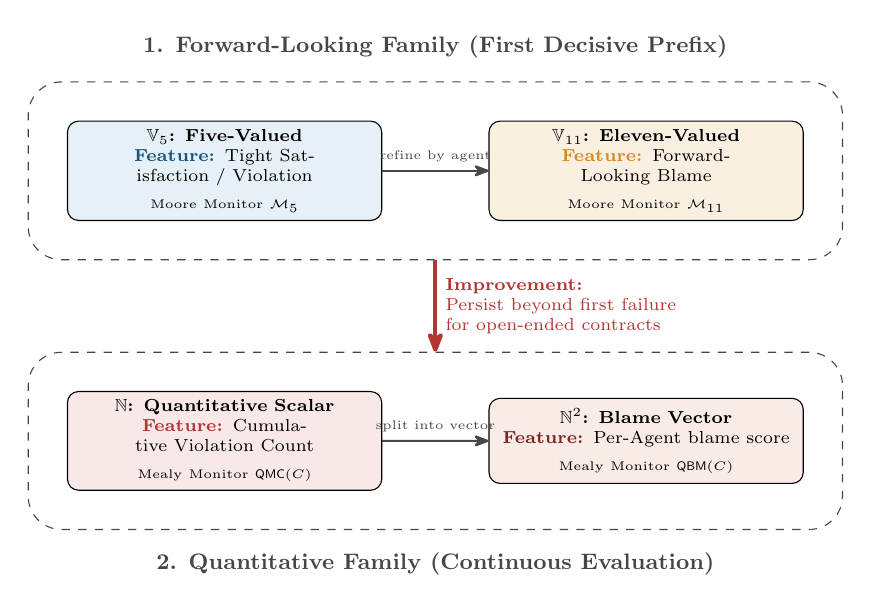
\begin{tikzpicture}[scale=0.9, transform shape,
    layer/.style={draw, rounded corners, text width=42mm, align=center, minimum height=12mm, font=\scriptsize},
    arr/.style={-{Stealth[round]}, thick, ConflictGray},
    fam/.style={draw=ConflictGray, dashed, rounded corners=12pt, inner sep=14pt},
    node distance=22mm and 15mm
  ]
    % Top Family (Forward-Looking)
    \node[layer, fill=SoftBlue] (v5) {\textbf{$\mathbb{V}_5$: Five-Valued}\\ \textcolor{ConflictBlue}{\textbf{Feature:}} Tight Satisfaction / Violation\\ \vspace{1mm}\tiny Moore Monitor $\mathcal{M}_5$};
    \node[layer, fill=SoftOrange, right=of v5] (v11) {\textbf{$\mathbb{V}_{11}$: Eleven-Valued}\\ \textcolor{ConflictOrange}{\textbf{Feature:}} Forward-Looking Blame\\ \vspace{1mm}\tiny Moore Monitor $\mathcal{M}_{11}$};
    \draw[arr] (v5) -- node[above,font=\tiny] {refine by agent} (v11);
    
    \node[fam, fit=(v5) (v11)] (fam1) {};
    \node[above=2mm of fam1.north, font=\small\bfseries, text=ConflictGray] {1. Forward-Looking Family (First Decisive Prefix)};
  
    % Bottom Family (Quantitative)
    \node[layer, fill=SoftRed, below=24mm of v5] (qn) {\textbf{$\mathbb{N}$: Quantitative Scalar}\\ \textcolor{ConflictRed}{\textbf{Feature:}} Cumulative Violation Count\\ \vspace{1mm}\tiny Mealy Monitor $\qmc(C)$};
    \node[layer, fill=SoftRed!70!SoftOrange, right=of qn] (qn2) {\textbf{$\mathbb{N}^2$: Blame Vector}\\ \textcolor{ConflictRed!70!black}{\textbf{Feature:}} Per-Agent blame score\\ \vspace{1mm}\tiny Mealy Monitor $\qbm(C)$};
    \draw[arr] (qn) -- node[above,font=\tiny] {split into vector} (qn2);
  
    \node[fam, fit=(qn) (qn2)] (fam2) {};
    \node[below=2mm of fam2.south, font=\small\bfseries, text=ConflictGray] {2. Quantitative Family (Continuous Evaluation)};
  
    % Improvement Arrow
    \draw[-{Stealth[round]}, line width=1.5pt, ConflictRed] (fam1.south) -- node[right,font=\scriptsize,align=left] {\textbf{Improvement:}\\Persist beyond first failure\\for open-ended contracts} (fam2.north);
  
  \end{tikzpicture}
  
  \vspace{5mm}
  \textbf{Result:} $\qsem{\pi,C} = n_1 + n_2$ \textemdash\ \emph{blame is a strict refinement of the violation count.}
  \end{frame}

% =====================================
% PART II — Slide 4
% =====================================
\begin{frame}{Tight Forward  Denotational Semantics}
\small
\begin{columns}[T,totalwidth=\textwidth]
\begin{column}{0.50\textwidth}
  \begin{block}{Two verdict domains}
    \footnotesize
    \begin{itemize}
      \item $\mathbb{V}_5=\{?,\topt,\bott,\topp,\botp\}$
      \item $\mathbb{V}_{11}=\{?,\topt,\topp\}\cup\{\bottp{S},\botpp{S}\mid S\subseteq\{1,2\}\}$
    \end{itemize}
  \end{block}
\textbf{Why it matters:} reparations and triggers switch exactly at the decisive prefix.
\end{column}
\begin{column}{0.46\textwidth}
  \begin{block}{Obligation example: $C=\obl[1]{\PAY}$}
    \footnotesize
    \[
    \begin{array}{lcl}
    \PAY^{(1)}\notin A &\Rightarrow& \mathbb{V}_5:\ \bott\\[2pt]
    \PAY^{(1)}\in A,\ \PAY^{(2)}\notin A &\Rightarrow& \mathbb{V}_5:\ \bott
    \end{array}
    \]
    In $\mathbb{V}_5$, both failures are just violations.
  \end{block}

  \begin{block}{$\mathbb{V}_{11}$ distinguishes blame}
    \footnotesize
    \[
    \begin{array}{lcl}
    \PAY^{(1)}\notin A &\Rightarrow& \bottp{\{1\}}\\[2pt]
    \PAY^{(1)}\in A,\ \PAY^{(2)}\notin A &\Rightarrow& \bottp{\{2\}}
    \end{array}
    \]
    Same frontier, but now we know who caused the violation.
  \end{block}
\end{column}
\end{columns}
\end{frame}


% =====================================
% PART II — Slide 6
% =====================================
\begin{frame}{Correct-by-Construction Moore Monitors}
\footnotesize
\begin{columns}[T,totalwidth=\textwidth]
\begin{column}{0.42\textwidth}
  \begin{center}
  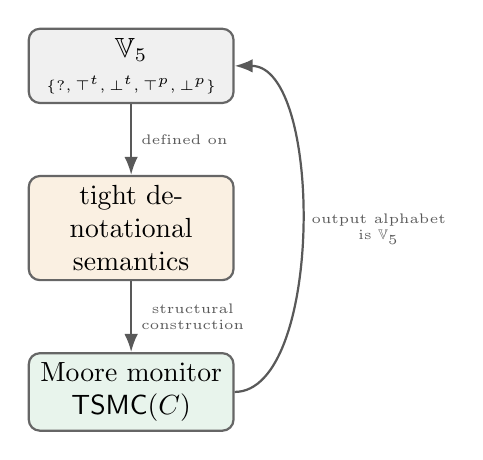
\begin{tikzpicture}[
    box/.style={rounded corners=4pt, draw=black!60, thick, minimum width=2.6cm, minimum height=0.9cm, align=center, text width=2.35cm},
    arr/.style={-{Latex[length=2.3mm]}, thick, black!65},
    lab/.style={font=\tiny, align=center}
  ]
    \node[box, fill=gray!12] (v5) {$\mathbb{V}_5$\\\tiny $\{?,\topt,\bott,\topp,\botp\}$};
    \node[box, fill=SoftOrange, below=9mm of v5] (sem) {tight denotational\\semantics};
    \node[box, fill=SoftGreen, below=9mm of sem] (mon) {Moore monitor\\$\tsmc(C)$};
    \draw[arr] (v5) -- node[right,lab] {defined on} (sem);
    \draw[arr] (sem) -- node[right,lab] {structural\\construction} (mon);
    \draw[arr] (mon.east) to[out=0,in=0,looseness=0.7] node[right,lab] {output alphabet\\is $\mathbb{V}_5$} (v5.east);
  \end{tikzpicture}
  \end{center}

 

\end{column}
\begin{column}{0.56\textwidth}
  \begin{block}{Example: Moore machine for $\obl[1]{\PAY}$}
  \centering
  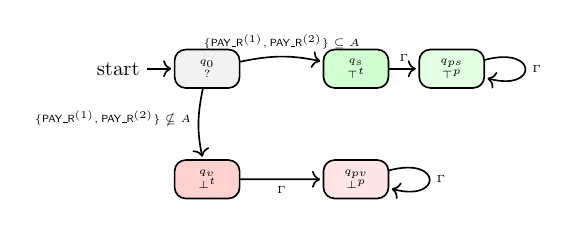
\begin{tikzpicture}[scale=0.75, transform shape,
    shorten >=1pt,auto,node distance=12mm and 14mm,semithick,
    every state/.style={rectangle,rounded corners,draw,minimum width=11mm,
      minimum height=6.5mm,inner sep=2.5pt,font=\tiny,align=center}
  ]
    \node[initial,state,fill=gray!10] (q0)  {$q_0$\\$?$};
    \node[state,fill=green!18,right=of q0] (qs)  {$q_s$\\$\topt$};
    \node[state,fill=red!18,below=of q0]   (qv)  {$q_v$\\$\bott$};
    \node[state,fill=green!10,right= 0.5cmof  qs] (qps) {$q_{ps}$\\$\topp$};
    \node[state,fill=red!10,right=of qv]   (qpv) {$q_{pv}$\\$\botp$};

    \path[->]
      (q0) edge[bend left=12] node[above,pos=0.5] {\tiny $\{\PAY^{(1)},\PAY^{(2)}\}\subseteq A$} (qs)
      (q0) edge[bend right=12] node[left,pos=0.42] {\tiny $\{\PAY^{(1)},\PAY^{(2)}\}\nsubseteq A$} (qv)
      (qs)  edge node[above] {\tiny $\Gamma$} (qps)
      (qv)  edge node[below] {\tiny $\Gamma$} (qpv)
      (qps) edge[loop right] node {\tiny $\Gamma$} (qps)
      (qpv) edge[loop right] node {\tiny $\Gamma$} (qpv);
  \end{tikzpicture}
  \end{block}

  \begin{block}{Construction}
    \begin{itemize}
      \item Construction à la Thomson.
      \item Conformance proof to the semantics.
    \end{itemize}
  \end{block}
\end{column}
\end{columns}
\end{frame}

% =====================================
% PART II — Slide 7
% =====================================
\begin{frame}{Quantitative violation $\qsem{}:\Gamma^* \times \cDL \to \mathbb{N}$}
\scriptsize
  \begin{block}{Two ingredients}
    $\LH(C)$ tells us \emph{which literal is currently in force}.
    \qquad
    $\Prog(\textcolor{orange!70!black}{\trace{A}},C)$ tells us \emph{how the contract evolves after the current event}.
  \end{block}

  \begin{block}{Fixpoint intuition}
    \[
    \qsem{\textcolor{orange!70!black}{\trace{A}}\cdot \textcolor{blue!70!black}{\pi}, C}
    =
    \textcolor{orange!70!black}{\underbrace{\qsem{\textcolor{orange!70!black}{\trace{A}},C}}_{\text{score now}}}
    +
    \textcolor{blue!70!black}{\underbrace{\qsem{\textcolor{blue!70!black}{\pi},\Prog(\textcolor{orange!70!black}{\trace{A}},C)}}_{\text{continue on the residual}}}
    \]
    \textcolor{orange!70!black}{Orange: score the current event.}
    \qquad
    \textcolor{blue!70!black}{Blue: continue with the residual contract.}
  \end{block}

  \begin{block}{Example}
    Let $C=\obl[1]{\PAY}\repair\obl[1]{\PAYF}$.
    \[
    \pi=\textcolor{orange!70!black}{\trace{A_1}}\cdot \textcolor{blue!70!black}{\trace{A_2}},
    \quad
    A_1=\{\OCC^{(1)}\},
    \quad
    A_2=\{\PAYF^{(12)}\}
    \]
    \[
    \begin{aligned}
    \textcolor{orange!70!black}{\trace{A_1}}:\;&
    \LH(C)=\obl[1]{\PAY},
    \quad
    \textcolor{orange!70!black}{\qsem{\trace{A_1},C}=1},
    \quad
    \textcolor{blue!70!black}{\Prog(\trace{A_1},C)=\obl[1]{\PAYF}}
    \\
    \textcolor{blue!70!black}{\trace{A_2}}:\;&
    \LH(\obl[1]{\PAYF})=\obl[1]{\PAYF},
    \quad
    \qsem{\trace{A_2},\obl[1]{\PAYF}}=0
    \end{aligned}
    \]
  
    \[
    \qsem{\pi,C}=1+0=1.
    \]
  \end{block}
\end{frame}

% =====================================
% PART II — Slide 8
% =====================================
\begin{frame}{Intuition for the Quantitative Violation Monitor $\qmc(C)$}
\footnotesize
\begin{columns}[T,totalwidth=\textwidth]
\begin{column}{0.48\textwidth}
  \begin{block}{Construction idea}
    Turn the denotational recursion into a Mealy machine:
    \[
    \qmc(C)=(Q,q_0,\Gamma,\delta,\lambda)
    \]
    where
    \begin{itemize}
      \item $Q=\rrcs{C}$ is the set of reachable residual contracts,
      \item $q_0=C$ is the initial residual,
      \item $\delta(q,A)=\Prog(\trace{A},q)$ updates the contract state,
      \item $\lambda(q,A)=\qsem{\trace{A},q}$ emits the local cost.
    \end{itemize}
  \end{block}

  \begin{block}{Finite state Mealy machine} 
    If $\rrcs{C}$ is finite, the monitor is finite too.
  \end{block}
\end{column}
\begin{column}{0.48\textwidth}
  \begin{block}{Execution view}
    \[
    q_0=C
    \xrightarrow{\trace{A_0}/\lambda(q_0,A_0)} q_1
    \xrightarrow{\trace{A_1}/\lambda(q_1,A_1)} q_2
    \xrightarrow{\ \cdots\ } q_n
    \]
    Each transition does two things:
    \begin{itemize}
      \item advance the residual contract by progression;
      \item output the score contributed by the current event.
    \end{itemize}
  \end{block}

  \begin{block}{Correctness takeaway}
    Along the unique run on $\pi$,
    \[
    \qscore(\qmc(C),\pi)
    =
    \sum_{i=0}^{n-1}\lambda(q_i,A_i)
    =
    \qsem{\pi,C}.
    \]
    So the monitor is an executable realization of the quantitative semantics.
  \end{block}
\end{column}
\end{columns}
\end{frame}

% =====================================
% SLIDE 21 — Contributions Summary
% =====================================
\begin{frame}{Summary of Contributions}
\small
\begin{columns}[T]
\begin{column}{0.48\textwidth}
  \begin{block}{\textcolor{ConflictBlue}{Conflict Analysis ($\TDDLfm$)}}
    \begin{enumerate}
      \item Formal machinery: interval-set logic, \dpnf, conflict calculus.
      \item Exact characterisation: $\text{unsat} \Leftrightarrow \cd(\phi) = 1$.
      \item Conflict density metric $\cd(\phi) \in [0,1]$.
      \item Sound \& complete conflict-free rewriting $\Namb(\phi)$.
      \item Complexity bounds \& conciseness analysis.
    \end{enumerate}
  \end{block}
\end{column}
\begin{column}{0.48\textwidth}
  \begin{block}{\textcolor{ConflictGreen}{Contract Monitoring (\cDL)}}
    \begin{enumerate}
      \item Attempt-based interaction model.
      \item \cDL logic with repetition, guards, triggers, reparation.
      \item 5-valued tight satisfaction semantics + Moore monitors.
      \item 11-valued forward blame semantics + blame monitors.
      \item Quantitative scalar ($\mathbb{N}$) and vector ($\mathbb{N}^2$) blame monitors.
      \item Full pipeline: denotational $\to$ operational, with conformance proofs.
    \end{enumerate}
  \end{block}
\end{column}
\end{columns}
\end{frame}

% =====================================
% SLIDE 22 — Outlook
% =====================================
\begin{frame}{Outlook \& Future Work}
\begin{columns}[T]
\begin{column}{0.48\textwidth}
  \textbf{Extending $\TDDLfm$:}
  \begin{itemize}
    \item Actions with \emph{duration}.
    \item Out to be (states).
    \item Conditional \& permission literals.
    \item More ontic conflicts types such as causality and resource conflicts.
  \end{itemize}
\end{column}
\begin{column}{0.48\textwidth}
  \textbf{Extending \cDL:}
  \begin{itemize}
    \item Algorithm and complexity proof for $\rrcs{C}$.
    \item $n$-agent generalisation ($\mathbb{N}^n$ blame vectors).
    \item Metric time instead of synchronous periods.
  \end{itemize}
\end{column}
\end{columns}

\vspace{5mm}
\centering
  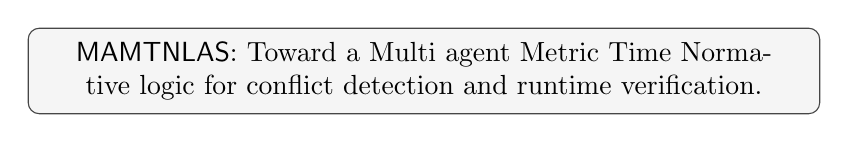
\begin{tikzpicture}
  \node[draw=ConflictGray,rounded corners,fill=gray!8,text width=0.8\textwidth,align=center,inner sep=5pt,font=\normalsize] {
  \textsf{MAMTNLAS}: Toward a Multi agent Metric Time Normative logic for conflict detection and runtime verification.
  };
\end{tikzpicture}

\vspace{4mm}
{\Large\bfseries Thank you! \quad Questions?}
\end{frame}

\appendix

% =====================================
% BACKUP SLIDE 1a — LUCO
% =====================================
\begin{frame}{Backup: Lowest Upper Common Operator (\LUCO)}
\small
\begin{columns}[T]
\begin{column}{0.52\textwidth}
  \begin{block}{Definition}
    Let $\mathsf{T}(\phi)$ be the Boolean syntax tree of $\phi$ (internal nodes $\sqcap,\sqcup$; leaves are literals).
    For literals $\ell_i,\ell_j$ each occurring once, $\LUCO_\phi(\ell_i,\ell_j)$ is the \emph{deepest} node $v$ that:
    \begin{enumerate}[(i)]
      \item is labeled $\sqcap$ or $\sqcup$;
      \item lies on both root-to-$\ell_i$ and root-to-$\ell_j$ paths;
      \item no proper descendant of $v$ satisfies (i) and (ii).
    \end{enumerate}
  \end{block}
  \medskip
  \textbf{Key insight:} Two literals can form a punctual conflict \emph{only} when $\LUCO = \sqcap$ (they must appear together in a product term).
\end{column}
\begin{column}{0.45\textwidth}
  \textbf{Example:} $\phi = \big((\ell_1 \sqcup \ell_2)\sqcap \ell_3\big)\sqcup\big(\ell_4 \sqcap \ell_5\big)$

  \begin{center}
  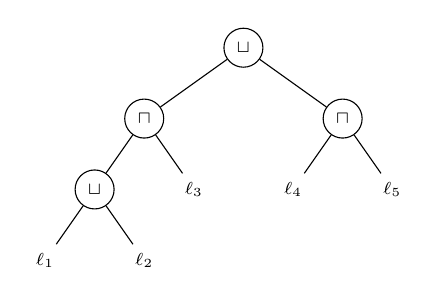
\begin{tikzpicture}[
    level distance=10mm,
    level 1/.style={sibling distance=28mm},
    level 2/.style={sibling distance=14mm},
    every node/.style={font=\scriptsize},
    op/.style={draw,circle,minimum size=5.5mm,inner sep=0.5mm},
    scale=0.9, transform shape
  ]
  \node[op] {$\sqcup$}
    child { node[op] {$\sqcap$}
      child { node[op] {$\sqcup$}
        child { node {$\ell_1$} }
        child { node {$\ell_2$} }
      }
      child { node {$\ell_3$} }
    }
    child { node[op] {$\sqcap$}
      child { node {$\ell_4$} }
      child { node {$\ell_5$} }
    };
  \end{tikzpicture}
  \end{center}

  \vspace{1mm}
  \footnotesize
  \renewcommand{\arraystretch}{1.15}
  \begin{tabular}{ll}
  $\LUCO(\ell_1,\ell_2)=\sqcup$ & (same branch, disj.)\\
  $\LUCO(\ell_1,\ell_3)=\sqcap$ & \textcolor{ConflictRed}{can conflict}\\
  $\LUCO(\ell_4,\ell_5)=\sqcap$ & \textcolor{ConflictRed}{can conflict}\\
  $\LUCO(\ell_1,\ell_4)=\sqcup$ & (cross-branch)\\
  \end{tabular}
\end{column}
\end{columns}

\vspace{3mm}
\centering
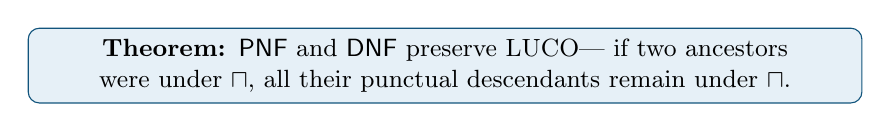
\begin{tikzpicture}
  \node[draw=ConflictBlue,rounded corners,fill=SoftBlue,text width=0.85\textwidth,align=center,inner sep=4pt,font=\small] {
  \textbf{Theorem:} $\pnf$ and $\dnf$ preserve \LUCO --- if two ancestors were under $\sqcap$, all their punctual descendants remain under $\sqcap$.
  };
\end{tikzpicture}
\end{frame}

% =====================================
% BACKUP SLIDE 1b — LAP
% =====================================
\begin{frame}{Backup: Literal Ancestor Preservation (\LAP)}
\small
\begin{columns}[T]
\begin{column}{0.52\textwidth}
  \begin{block}{Definition}
    $\phi'$ satisfies \LAP of $\phi$ if there is a mapping from literals in $\phi'$ to literals in $\phi$ such that:
    \begin{enumerate}[(i)]
      \item \textbf{Downward:} every $\ell'$ in $\phi'$ has ancestor $\ell$ in $\phi$ with same modality, action, and $\is(\ell') \subseteq \is(\ell)$.
      \item \textbf{Upward:} for every $\ell$ in $\phi$, its descendants $\{\ell_1',\dots,\ell_n'\}$ in $\phi'$ recombine under their \LUCO to reconstruct $\ell$.
    \end{enumerate}
  \end{block}
  \medskip
  \textbf{Purpose:} No new time points are created, none are lost. Normalization only \emph{refines} literals into punctual pieces.
\end{column}
\begin{column}{0.45\textwidth}
  \textbf{Example:}
  \[
  \phi := \ob{\{[2,3]\}}{a} \;\sqcap\; \forbb{\{[2,4]\}}{a}
  \]
  After $\pnf$:
  \[
  \phi' := \big(\ob{\{[2,2]\}}{a} \sqcup \ob{\{[3,3]\}}{a}\big) \sqcap \forbb{\{[2,2]\}}{a} \sqcap \forbb{\{[3,4]\}}{a}
  \]

  \footnotesize
  \textbf{Downward \checkmark:}
  \begin{itemize}\setlength\itemsep{1pt}
    \item $\ob{\{[2,2]\}}{a}, \ob{\{[3,3]\}}{a}$ descend from $\ob{\{[2,3]\}}{a}$
    \item $\forbb{\{[2,2]\}}{a}, \forbb{\{[3,4]\}}{a}$ descend from $\forbb{\{[2,4]\}}{a}$
  \end{itemize}
  \textbf{Upward \checkmark:}
  \begin{itemize}\setlength\itemsep{1pt}
    \item $\ob{\{[2,2]\}}{a} \sqcup \ob{\{[3,3]\}}{a} \equiv \ob{\{[2,3]\}}{a}$
    \item $\forbb{\{[2,2]\}}{a} \sqcap \forbb{\{[3,4]\}}{a} \equiv \forbb{\{[2,4]\}}{a}$
  \end{itemize}
\end{column}
\end{columns}

\vspace{3mm}
\centering
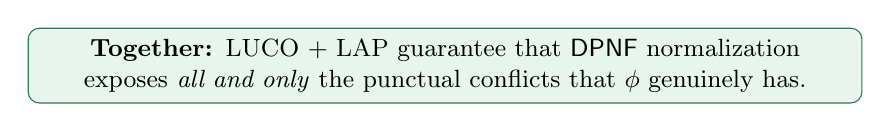
\begin{tikzpicture}
  \node[draw=ConflictGreen,rounded corners,fill=SoftGreen,text width=0.85\textwidth,align=center,inner sep=4pt,font=\small] {
  \textbf{Together:} \LUCO + \LAP guarantee that $\dpnf$ normalization exposes \emph{all and only} the punctual conflicts that $\phi$ genuinely has.
  };
\end{tikzpicture}
\end{frame}

% =====================================
% BACKUP SLIDE 2 — Examples of Repair
% =====================================
\begin{frame}{Backup: Conflict-Free Rewriting — Positive \& Negative Examples}
\small
\textbf{After conflict extraction:} prune all conflicting product terms $\Rightarrow$ $\Namb(\phi)$.

\medskip
\begin{columns}[T]
\begin{column}{0.50\textwidth}
  \begin{block}{\textcolor{ConflictGreen}{Positive: Compact rewriting exists}}
    \[
    \UC_2' := \ob{\{[9,16]\}}{\delAtPark} \sqcap \underbrace{\forbb{\{[10,14]\}}{\delAtPark}}_{\SR}
    \sqcap \underbrace{\forbb{\{[2,4],[8,24]\}}{\delAtGate}}_{\MA}
    \]
    Only times $t\!\in\!\{9,15,16\}$ are conflict-free.

    Verbose $\Namb(\UC_2')$ has size $94$, but merging via \textbf{ObDis}:
    \[
    \UC_2'' := \ob{\{[9,9],[15,16]\}}{\delAtPark} \sqcap \SR \sqcap \MA
    \]
    Size $18$ vs.\ original $16$. {\color{ConflictGreen}\checkmark}
  \end{block}
\end{column}
\begin{column}{0.47\textwidth}
  \begin{block}{\textcolor{ConflictRed}{Negative: Exponential blow-up}}
    \[
    \phi := \ob{\{[0,3]\}}{\mathsf{a}} \sqcap \ob{\{[0,3]\}}{\mathsf{b}} \sqcap \ob{\{[0,3]\}}{\mathsf{c}}
    \]
    Three obligations over 4 time points.
    \vspace{1mm}
    \begin{center}
    \renewcommand{\arraystretch}{1.2}
    \begin{tabular}{lc}
    \hline
    \textbf{Step} & \textbf{Size} \\\hline
    $\phi$ & 18 \\
    $\pnf(\phi,3)$ & 59 \\
    $\dnf(\pnf(\phi,3))$ & 959 \\
    $\Namb(\phi)$ (24 PT) & 359 \\\hline
    Blow-up & $\approx 20\times$
    \end{tabular}
    \end{center}
    \vspace{1mm}
    No compact rewrite exists: all 24 survivors need pairwise distinct time points. {\color{ConflictRed}Conflict calculus preferred.}
  \end{block}
\end{column}
\end{columns}
\end{frame}

% =====================================
% BACKUP SLIDE 3 — Conflict Calculus
% =====================================
\begin{frame}{Backup: Conflict Calculus for $\TDDLfm$}
\small
Eleven inference rules for big-step reasoning — no $\dpnf$ expansion required.

\vspace{2mm}
\begin{center}
\footnotesize
\renewcommand{\arraystretch}{1.35}
\begin{tabular}{|l|l|l|}
\hline
\textbf{Rule} & \textbf{Condition} & \textbf{Conclusion} \\\hline
\textbf{(O-Union)} & $\is = \is_1 \cup \is_2$ & $\ob{\is_1}{a} \sqcup \ob{\is_2}{a} \equiv \ob{\is}{a}$ \\\hline
\textbf{(F-Union)} & $\is = \is_1 \cup \is_2$ & $\forbb{\is_1}{a} \sqcup \forbb{\is_2}{a} \equiv \forbb{\is}{a}$ \\\hline
\textbf{(Distr1L)} & & $\phi_1 \sqcap (\phi_2 \sqcup \phi_3) \equiv (\phi_1 \sqcap \phi_2) \sqcup (\phi_1 \sqcap \phi_3)$ \\\hline
\textbf{($\bm{\equiv\sqcap}$)} & $\phi_1 \equiv \phi_1'$ & $\phi_1 \sqcap \phi_2 \equiv \phi_1' \sqcap \phi_2$ \\\hline
\textbf{($\bm{\bot\equiv}$)} & $\phi \equiv \phi',\; \phi' \vdash \bot$ & $\phi \vdash \bot$ \\\hline
\textbf{($\bm{\bot\sqcap}$)} & $\phi \vdash \bot$ & $\phi \sqcap \phi' \vdash \bot$ \\\hline
\textbf{($\bm{\bot\sqcup}$)} & $\phi \vdash \bot,\; \phi' \vdash \bot$ & $\phi \sqcup \phi' \vdash \bot$ \\\hline
\textbf{($\bm{\sqcup\bot}$)} & $\phi' \vdash \bot$ & $\phi \sqcup \phi' \equiv \phi$ \\\hline
\textbf{(T-DeoConf)} & $\is \subseteq \is'$ & $\ob{\is}{a} \sqcap \forbb{\is'}{a} \vdash \bot$ \\\hline
\textbf{(P-DeoConf)} & $\is \cap \is' \neq \emptyset,\; \is \not\subset \is'$ & $\ob{\is}{a} \sqcap \forbb{\is'}{a} \equiv \ob{\is \!\setminus\! \is'}{a} \sqcap \forbb{\is'}{a}$ \\\hline
\textbf{(OntConf)} & $|\is| <_\infty |\{a_1,\dots,a_n\}|$ & $\bigsqcap_{i} \ob{\is}{a_i} \vdash \bot$ \\\hline
\end{tabular}
\end{center}

\vspace{2mm}
\textbf{Use case $\UC = \UC_1' \sqcup \UC_2'$:}
\begin{itemize}
  \item \textbf{(T-DeoConf):} $\ob{\{[9,16]\}}{\delAtGate} \sqcap \forbb{\{[2,4],[8,24]\}}{\delAtGate} \vdash \bot$
  since $[9,16]\subseteq [2,4]\cup[8,24]$
  $\;\Rightarrow\; \UC_1' \vdash \bot$
  \item \textbf{(P-DeoConf):} $\ob{\{[9,16]\}}{\delAtPark} \sqcap \forbb{\{[10,14]\}}{\delAtPark} \equiv \ob{\{[9,9],[15,16]\}}{\delAtPark} \sqcap \forbb{\{[10,14]\}}{\delAtPark}$
  \item \textbf{($\bm{\sqcup\bot}$):} $\UC \equiv \UC_2'$ (the conflict-free refinement).
\end{itemize}
\end{frame}

% =====================================
% BACKUP SLIDE 4a — Timed Words → Periodic Set Traces
% =====================================
\begin{frame}{Backup: Step 1 — Metric-Timed Traces $\to$ Periodic Set Traces}
\small

\textbf{Input:} Raw metric-timed traces over 120 days (tenant = agent 1, landlord = agent 2).
\begingroup\footnotesize
\[
\begin{aligned}
\tau_1 &= \langle(\textsf{pay\_rent},5),\;(\textsf{start\_occ},35),\;(\textsf{pay\_rent},36),\;(\textsf{pay\_rent\_f},95)\rangle\\
\tau_2 &= \langle(\textsf{grant\_occ},1),\;(\textsf{ack\_pay},6),\;(\textsf{ack\_pay},37),\;(\textsf{ref\_pay},95),\;(\textsf{change\_lock},96)\rangle
\end{aligned}
\]
\endgroup

\begin{center}
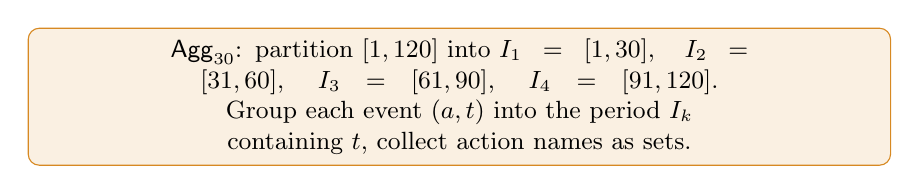
\begin{tikzpicture}
  \node[draw=ConflictOrange,rounded corners,fill=SoftOrange,text width=0.88\textwidth,align=center,inner sep=4pt,font=\small] {
  $\mathsf{Agg}_{30}$: partition $[1,120]$ into $I_1\!=\![1,30],\; I_2\!=\![31,60],\; I_3\!=\![61,90],\; I_4\!=\![91,120]$.\\
  Group each event $(a,t)$ into the period $I_k$ containing $t$, collect action names as sets.
  };
\end{tikzpicture}
\end{center}

\textbf{Output:} Periodic set traces $\pi_1, \pi_2$:
\begingroup\footnotesize
\[
\begin{aligned}
\pi_1 &= \langle
  \underbrace{\{\textsf{pay\_rent}\}}_{I_1},\;
  \underbrace{\{\textsf{start\_occ},\;\textsf{pay\_rent}\}}_{I_2},\;
  \underbrace{\emptyset}_{I_3},\;
  \underbrace{\{\textsf{pay\_rent\_f}\}}_{I_4}
\rangle\\[3pt]
\pi_2 &= \langle
  \underbrace{\{\textsf{grant\_occ},\;\textsf{ack\_pay}\}}_{I_1},\;
  \underbrace{\{\textsf{ack\_pay}\}}_{I_2},\;
  \underbrace{\emptyset}_{I_3},\;
  \underbrace{\{\textsf{ref\_pay},\;\textsf{change\_lock}\}}_{I_4}
\rangle
\end{aligned}
\]
\endgroup

\vspace{1mm}
\textbf{Key property:} Within each period, temporal ordering is abstracted away --- only \emph{presence} matters.
Between periods, the sequential structure is preserved by the index $k$.
\end{frame}

% =====================================
% BACKUP SLIDE 4b — Collaboration Alphabet + Tagged Traces
% =====================================
\begin{frame}{Backup: Step 2 — Collaboration Alphabet \& Tagged Traces}
\small

\textbf{Enabler/Blocker mapping} (from the contract specification):
\begingroup\footnotesize
\[
\begin{array}{r@{\;=\;\{}l@{\}}l}
E_1(\PAY) & \textsf{pay\_rent}   & E_2(\PAY) = \{\textsf{ack\_pay}\},\quad B_2(\PAY) = \{\textsf{ref\_pay}\}\\
E_1(\PAYF) & \textsf{pay\_rent\_f} & \\
E_1(\OCC) & \textsf{start\_occ}  & E_2(\OCC) = \{\textsf{grant\_occ}\},\quad B_2(\OCC) = \{\textsf{change\_lock}\}
\end{array}
\]
\endgroup

\begin{center}
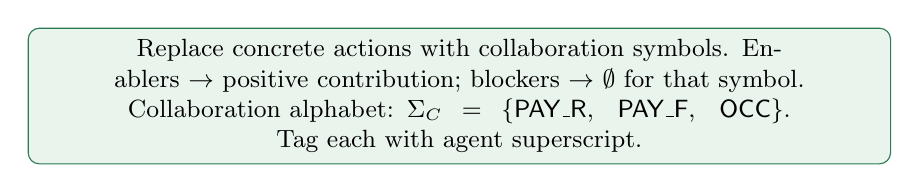
\begin{tikzpicture}
  \node[draw=ConflictGreen,rounded corners,fill=SoftGreen,text width=0.88\textwidth,align=center,inner sep=4pt,font=\small] {
  Replace concrete actions with collaboration symbols. Enablers $\to$ positive contribution; blockers $\to$ $\emptyset$ for that symbol.\\
  Collaboration alphabet: $\Sigma_C = \{\PAY,\;\PAYF,\;\OCC\}$. Tag each with agent superscript.
  };
\end{tikzpicture}
\end{center}

\textbf{Output:} Tagged collaboration traces $\pi_1^C, \pi_2^C$:
\begingroup\footnotesize
\[
\begin{aligned}
\pi_1^C &= \langle
  \underbrace{\{\PAY^{(1)}\}}_{I_1},\;
  \underbrace{\{\OCC^{(1)},\;\PAY^{(1)}\}}_{I_2},\;
  \underbrace{\{\OCC^{(1)}\}}_{I_3},\;
  \underbrace{\{\PAYF^{(1)}\}}_{I_4}
\rangle\\[3pt]
\pi_2^C &= \langle
  \underbrace{\{\OCC^{(2)},\;\PAY^{(2)}\}}_{I_1},\;
  \underbrace{\{\OCC^{(2)},\;\PAY^{(2)}\}}_{I_2},\;
  \underbrace{\{\OCC^{(2)}\}}_{I_3},\;
  \underbrace{\emptyset}_{I_4}
\rangle
\end{aligned}
\]
\endgroup

\vspace{1mm}
\textbf{Reading per month:}
\begin{itemize}\setlength\itemsep{1pt}
  \item $I_1$: Tenant pays rent; landlord grants occupation and accepts payment.
  \item $I_2$: Tenant pays and occupies; landlord allows both.
  \item $I_3$: Tenant keeps occupying but does not pay; landlord still allows occupation.
  \item $I_4$: Tenant pays late (\PAYF); \textcolor{ConflictRed}{landlord blocks \PAY and \OCC $\Rightarrow \emptyset$ (landlord blamed)}.
\end{itemize}
\end{frame}

\end{document}
